\startsection{Formulas}

\subsection*{Geometry}

Area of a regular polygon: $0.5ap$, where $a$ is the apothem (line from the center of the polygon to the midpoint of one of the sides) and $p$ is the perimeter

\textbf{Triangles}

Height $= a \sin(\theta)$, where $a$ is area

Area of an equilateral triangle $= \frac{\sqrt{3}}{4} s^2$, where $s$ is the side length

Area $= 0.5ab \sin(C)$ (using the Law of Sines triangle)

Heron's formula: The area of a triangle with side lengths $a$, $b$, and $c$ and semi-perimeter $s = \frac{a+b+c}{2}$ is $A = \sqrt{s (s-a) (s-b) (s-c)}$.

Area = $\displaystyle \Bigg\lvert \frac{A_x (B_y - C_y) + B_x (C_y - A_y) + C_x (A_y - B_y)}{2} \Bigg\rvert$, where $A$, $B$, and $C$ are the xy points

Centroid: $(X, Y)$ where $\displaystyle X = \frac{x_1 + x_2 + x_3}{3}$ and $\displaystyle Y = \frac{y_1 + y_2 + y_3}{3}$

\textbf{Circular segment}

\begin{center}
    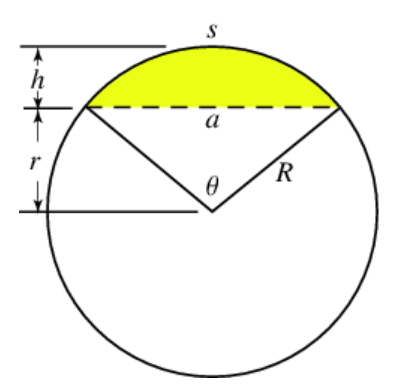
\includegraphics[scale=0.5]{math/img/circ_seg.png}
\end{center}

Radius: $R = r + h$

Arc length: $s = R \theta$

Height: $r = R \cos(\frac{1}{2} \theta) = \frac{1}{2} a \cot(\frac{1}{2} \theta) = \frac{1}{2} \sqrt{4 R^2 - a^2}$

Chord length: $a = 2R \sin(\frac{1}{2} \theta) = 2r \tan (\frac{1}{2} \theta) = 2 \sqrt{R^2 - r^2} = 2 \sqrt{h (2R - h)}$

Angle: $\theta = \frac{s}{R} = 2 \cos^{-1}(\frac{r}{R}) = 2 \tan^{-1}(\frac{a}{2r}) = 2 \sin^{-1}(\frac{a}{2R})$

Area: $A = \frac{1}{2} R^2 (\theta - \sin (\theta)) = \frac{1}{2} (Rs - ar) = R^2 \cos^{-1}(\frac{r}{R}) - r \sqrt{R^2 - r^2} = R^2 \cos^{-1}(\frac{R-h}{R}) - (R-h)\sqrt{2Rh - h^2}$

\textbf{Right circular cone}

Volume $= \frac{\pi r^2 h}{3}$

Lateral surface area $= \pi r \sqrt{r^2 + h^2}$

Total surface area $= Lateral + \pi r^2$

\textbf{Sphere}

Volume $= \frac{4}{3} \pi r^3$

Surface area $= 4 \pi r^2$

\textbf{General polygons}

Number the vertexes of the polygon, going either clockwise or counterclockwise.

$$\text{Area } = \Bigg\lvert \frac{(x_1 y_2 - y_1 x_2) + (x_2 y_3 - y_2 x_3) + ... + (x_n y_1 - y_n x_1)}{2} \Bigg\rvert$$

\subsection*{Permutations and combinations}

Combinations, no repetition: $\displaystyle \binom{n}{k} = \frac{n!}{k! (n-k)!}$

Combinations, with repetition: $\displaystyle \binom{n + k - 1}{k} = \frac{(n+k-1)!}{k! (n-1)!}$

Permutations, no repetition: $\displaystyle \frac{n!}{(n-k)!}$

Permutations, with repetition: $n^k$

\subsection*{Trigonometry}

\textbf{Law of Sine}

Use with $A, B, a$ (AAS), $A, c, B$ (ASA), and $a, b, A$ (SSA)

$$\frac{a}{\sin(A)} = \frac{b}{\sin(B)} = \frac{c}{\sin(C)} \formsep h = b \sin(A)$$

Ambiguous case: two sides and an angle \textit{not} between

\begin{itemize}
    \item Case 1: $\theta > 90^\circ$
    \begin{itemize}
        \item $opposite < adjacent$: no possible triangles
        \item $opposite > adjacent$: 1 possible triangle
    \end{itemize}
    \item Case 2: $\theta < 90^\circ$
    \begin{itemize}
        \item $opposite = height$: 1 possible right triangle
        \item $opposite < height$: no possible triangles
        \item $opposite > height$:
        \begin{itemize}
            \item $opposite < adjacent$: 1 possible triangle
            \item $opposite > adjacent$: 2 possible triangles
        \end{itemize}
    \end{itemize}
\end{itemize}

\subsection*{Law of Cosine}

Use with $a, C, b$ (SAS) and $a, b, c$ (SSS)

Note: Find the largest angle first. Find the smallest angle second. (This includes given angles. eg. if you are given SAS, find the smallest angle.)

$$a^2 = b^2 + c^2 - 2bc \cos(A)$$

\newpage